 \newcolumntype{C}[1]{>{\centering\arraybackslash}p{#1}}

\section{Ryšio mažame lauke technologija}

\subsection{Radijo dažnio identifikavimo technologija}
Radijo dažnio identifikavimas (angl. \textit{Radio-frequency identification}) (toliau- RFID) tai viena iš bevielio komunikavimo technologijų, kuri yra paremta elektromagnetinių bangų spektro dažniais, kurie padeda identifikuoti unikalius objektus. Pirmieji RFID panaudojo Britų armijos karininkai Antrajame pasauliniame kare, jie šią technologiją naudojo identifikuoti armijai priklausančius objektus, t.y. lėktuvus, radarus ir kt. \cite{Motlagh2012}. RFID sukuria vienos krypties arba dviejų krypčių bevielį duomenų srautą. Duomenų perdavime dalyvauja 2 aktoriai - žyma (angl. \textit{tag}) ir skaitytuvas (angl. \textit{reader}) \cite{Igoe2014}. Skaitytuvas inicijuoja komunikavimą, sukurdamas elektromagnetinio lauko bangas, ir laukia atsakymo iš žymos. Žyma priima skaitytuvo komunikavimo užklausą ir grąžina rezultatą. Žemiau pateiktoje diagramoje (žiūrėti 2 pav.) pavaizduota RFID sistem. Šią sistemą bei daugelį kitų RFID sistemų sudaro šie 3 pagrindiniai komponentai \cite{Hunt2006}: 
\begin{enumerate}
    \item \textbf{Žyma}, taip pat dar vadinama siųstuvu. Žyma yra sudaryta iš semi-konduktoriaus mikroschemos, antenos. Taip pat kartais žyma turi vidinį maitinimo šaltinį - bateriją;
    \item \textbf{Skaitytuvas}, jis yra sudarytas iš antenos, radjo bangų dažnių modulio, kuris skirtas siųsti ir gauti signalus iš žymos, ir valdymo modulio;
    \item \textbf{Valdiklis} (angl. \textit{controller}), taip pat dar vadinamas pagrindiniu kompiuteriu (angl. \textit{host}). Dažniausiai tai yra kompiuteris, kuriame yra duomenų bazė ir valdymo programinė įranga.
\end{enumerate}

\begin{figure}[H]
    \centering
    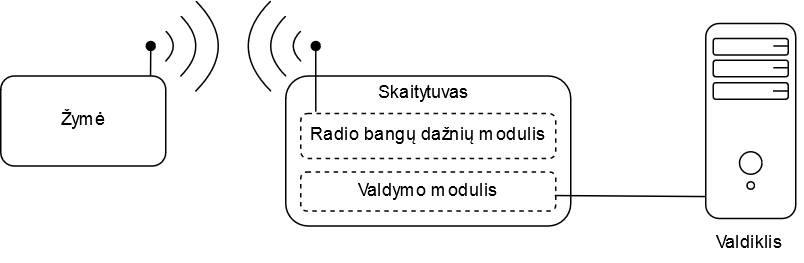
\includegraphics[scale=0.42]{images/RFID}
    \caption{RFID sistemos komponentų diagrama} 
\end{figure}

RFID įrenginių komunikavimas yra skirstomos į 2 tipus \cite{Igoe2014}:
\begin{enumerate}
    \item Aktyvus komunikavimo tipas. Šiam tipui priklauso tos RFID technologijos, kurių aktoriai turi savo nuosavus energijos šaltinius. Kuomet žyma siunčia rezultatą skaitytuvui, jis naudoja energiją, kuri yra gaunama iš nuosavo maitinimo šaltinio;
    \item Pasyvus komunikavimo tipas. Šiam tipui priklauso tos RFID technologijos, kurių vienas iš aktorių neturi nuosavo energijos šaltinio, t.y. žyma - neturi, o siųstuvas turi. Tam, kad žyma išsiųstų rezultatą, ji reikiamą energiją gauna iš iniciatoriaus sukurto magnetinio lauko.
\end{enumerate}
Lentelėje (žiūrėti 2 lentelę) pateikiamas aktyvios ir pasyvios žymos palyginimas.

\begin{table}[H]
    \centering
    \renewcommand{\arraystretch}{1,2}
    \caption{Aktyvios ir pasyvios RFID žymos palyginimas}

    \begin{tabular}{| p{10em} | p{12em} | p{12em} |}\hline
        \backslashbox[10em]{Ypatybės}{Tipai}
        &\makebox[12em]{Aktyvus}&\makebox[12em]{Pasyvus}\\\hline
        Maitinimo šaltinis & Vidinis & Išorinis\\\hline
        Skaitymo diapazonas & Didelis - iki 100 metrų & Nėra didelis - iki 3 metrų   \\\hline
        Žymos veikimo laikas & Kadangi žyma turi vidinį maitinimo šaltinį, jis nuolatos būna veikimo būsenoje & Žyma pradeda veikti tik tuomet, kai skaitytuvas inicijuoja komunikavimą \\\hline
        Magnetinio lauko stiprumas & Magnetinis laukas nėra stiprus, nes žyma naudoja vidinę energiją tam, kad išsiųstų signalą  & Sukuriamas stiprus magnetinis laukas, nes šio magnetinio lauko dėka žyma įgyja energijos išsiųsti signalą \\\hline
        Naudojimo terminas & Naudojimo terminas priklauso nuo maitinimo šaltinio galiojimo termino & Naudojimo terminas nėra apibrėžtas \\\hline
        Saugomų duomenų dydis &  Didesnis, dažnu atveju 128 kilobaitai (angl \textit{Kilobyte}) & Mažas, dažniausiai 128 baitai (angl. \textit{Byte})  \\\hline
        Dydis & Dydis priklauso nuo maitinimo šaltinio dydžio & Mažas \\\hline
        Kaina & Brangesnis nei pasyvus & Brangesnis nei aktyvus \\\hline
    \end{tabular}
\end{table}

RFID technologijos charakteristikos nėra pastovios, šios technologijos savybėm didžiausią įtaką daro parinktas elektromagnetinės bangos dažnis, kuris yra naudojamas komunikavimui tarp skaitytuvo ir žymos. Todėl kuriant sistemą, kuri yra paremta RFID technologija, svarbu pasirinkti tinkamą bangos dažnį. RFID technologijos naudojami elektromagnetinių bangų dažniai: kilometrinės bangos žemieji dažniai (toliau - ŽD), dekametrinės bangos aukštieji dažniai  (toliau - AD), decimetrinės bangos ultra aukšti dažniai (toliau - UAD) ir mikrobangų dažniai. Šių dažnių naudojimą RFID sistemose aprašo ISO ir IEC standartai. Elektromagnetinių bangų dažniai daro įtaką šioms RFID savybės \cite{Hunt2006}:
\begin{enumerate}
    \item \textbf{Skaitymo diapazonas}. Žemesnių bangų dažnių RFID skaitymo diapazonas būna mažas. Aukštesnių bangų dažnių RFID skaitymo diapazonas yra didesnis, ypač jeigu naudojamas aktyvus RFID tipas;
    \item \textbf{Aktyvus ir pasyvus RFID}. Istoriškai pasyvus RFID naudodavo ŽD ir AD dažnius, o aktyvus - UAD ir mikrobangų dažnius, tačiau šiuo metu abiejų tipų RFID gali naudotis aukštesnius dažnius, t.y. UAD ir mikrobangų dažnius;
    \item \textbf{Radijo dažnių trukdžiai}. Žemesnių dažnių RFID yra labiau atsparūs interferencijai, nei aukštesnių dažnių RFID;
    \item \textbf{Vandens ir metalo įtaka}. Mikrobangos ir UAD turi didesnę tikimybę būti sugertiems skysčio, todėl šių dažnių RFID nėra tinkamas naudoti šlapiem objektams. Kadangi metalas atspindi elektromagnetines bangas, jos negali prasiskverbti pro jį, tačiau net šalia esantis metalas taip pat gali atspindėti elektromagnetines bangas, todėl tiek aukštesnio dažnio, tiek žemesnio dažnio bangoms metalas daro įtaką. Žemesnio dažnio bangos yra paveikiamos metalo mažiau nei aukštesnio.
\end{enumerate}
Žemiau pavaizduotoje lentelėje (žiūrėti 3 lentelę), pateikiamos RFID tipų naudojami elektromagnetiniai bangų dažniai, jų naudojimą apibrėžiantys standartai \cite{Caglar2016}.

\begin{table}[!ht]
    \centering
    \caption{Aktyvaus ir pasyvaus RFID komunikavimo tipų palyginimas}
    \renewcommand{\arraystretch}{1,5}
    \begin{tabular}{m{9em}m{8em}m{8em}m{8em}} 
        \hline
        Elektromagnetinė banga            & Bangos dažniai    & RFID tipas    &Standartai   \\ 
        \hline
        ŽD                     & 125-134.2 KHz & Pasyvus & ISO 11784 \par ISO/IEC 18000-2A \par ISO/IEC 18000-2B   \\ 
        \hline
        AD                     & 13.56 MHz & Pasyvus  &  ISO 18000-3 \par ISO/IEC 15693 \\ 
        \hline
        \multirow{2}{*}{UAD} & 433 MHz       & Aktyvus   &  ISO 18000-7    \\ 
        \cline{2-4}
                                & 860 ir 915 MHz      &  Pasyvus ir Aktyvus  &  ISO 18000-6A \par ISO 18000-6B \par ISO 18000-6C    \\ 
        \hline
        Mikrobangos                       & 2.45 ir 5.8 GHz         & Pasyvus ir Aktyvus &  ISO 18000-4  \\
        \hline
    \end{tabular}
\end{table}

\subsection{Artimojo lauko ryšys}
\subsubsection{Sąvoka}
ALR tai bevielio komunikavimo technologija, ši technologija yra pagrįsta anksčiau minėtos RFID technologijos standartais ir interfeisais. Todėl įrenginiai, kurie paremti ALR technologija, gali komunikuoti su dauguma RFID technologijos įrenginių \cite{Motlagh2012}. ALR įrenginiai tarpusavyje komunikuoja 13,56 MHz elektromagnetinių bangų dažniu, duomenų perdavimo greitis svyruoja nuo 106 kilobitų per sekundę iki 424 kilobitų per sekundę \cite{whitepapaer}. Maksimalus veikimo atstumas tarp ALR įrenginių literatūroje minimas ne vienodas. Apibendrinus literatūros šaltinius, maksimalus veikimo atstumas yra tarp 4 centimetrų ir 20 centimetrų \cite{whitepapaer} \cite{Motlagh2012} \cite{Leora1980}. Pagrindiniai skirtumai tarp RFID ir ALR technologijų \cite{Leora1980}:
\begin{enumerate}
    \item Komunikavimo atveju, atstumas tarp ALR įrenginių turi būti mažas, o RFID technologijoje naudojant aktyvias žymes, atstumas gali būti žymiai didesnis;
    \item ALR technologijoje naudojamos tik pasyvios žymės, o RFID technologijoje naudojamos tiek aktyvios, tiek pasyvios žymės;
    \item Dėl to, kad komunikavimo atstumas yra mažas, duomenų perdavimas laikomas saugesniu nei RFID;
    \item Dėl to, kad komunikavimo atstumas yra mažas, skaitytuvas komunikuoja su norima žyma, todėl mažėja tikimybė jog skaitytuvo veikimo lauke atsiras keletą žymų.
\end{enumerate}
 

\subsubsection{Duomenų apsikeitimo specifikacija}
ALR duomenų apsikeitimo formatas (angl. \textit{NFC Data Exchange Format}) (toliau - NDEF) tai standartas, kuris nusako duomenų apsikeitimo formatą tarp ALR įrenginio ir ALR žymės arba tarp dviejų ALR įrenginių \cite{Leora1980}. Komunikavimo metu, siunčiama NDEF žinutė, kurią sudaro vienas arba daugiau NDEF įrašų (angl. \textit{records}) (žiūrėti 3 pav.). NDEF įrašą sudaro antraštė (angl. \textit{header}) ir informacija (angl. \textit{payload}), kurios dydis yra iki 2\textsuperscript{32}-1 baitų \cite{NFCForum2006}. Norint talpinti didesnį kiekį duomenų, NDEF įrašai gali būti apjungti. Kadangi NDEF žinutę gali sudaryti daugiau nei vienas įrašas, svarbu indikuoti žinutės rėžius, todėl pirmasis įrašas žinutės eilėje turi žinutės pradžios indikatorių, o paskutinis įrašas - žinutės pabaigos indikatorių.

\begin{figure}[H]
    \centering
    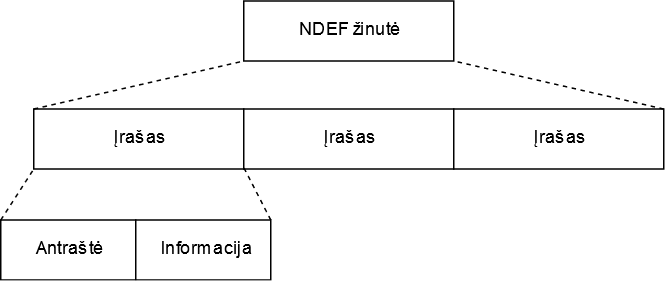
\includegraphics[scale=0.5]{images/NDEF}
    \caption{NDEF žinutės sudedamosios dalys} 
\end{figure}


Žemiau pateiktoje lentelėje (žiūrėti 4 lentelę) yra nurodoma NDEF žinutės įrašą sudarantys laukai. 

\begin{table}[H]
    \centering
    \caption{NDEF žinutės įrašas \cite{NFCForum2006} }
    \renewcommand{\arraystretch}{1,7}
    \begin{tabular}{C{2em}C{2em}C{2em}C{2em}C{2em}C{2em}C{2em}C{2em}l}
        7                         & 6                        & 5                       & 4                       & 3                       & 2 & 1 & 0                 &                        \\ 
        \hline
        \multicolumn{1}{|c|}{ŽPR} & \multicolumn{1}{c|}{ŽPA} & \multicolumn{1}{c|}{DD} & \multicolumn{1}{c|}{TĮ} & \multicolumn{1}{c|}{IB} & \multicolumn{3}{c|}{ĮTF } & \parbox[t]{2mm}{\multirow{6}{*}{\rotatebox[origin=c]{270}{Antraštė}}}  \\ 
        \cline{1-8}
        \multicolumn{8}{|c|}{Įrašo tipo dydis}                                                                                                                         &                        \\ 
        \cline{1-8}
        \multicolumn{8}{|c|}{Informacijos dydis}                                                                                                                       &                        \\ 
        \cline{1-8}
        \multicolumn{8}{|c|}{ID dydis}                                                                                                                                 &                        \\ 
        \cline{1-8}
        \multicolumn{8}{|c|}{Įrašo tipas}                                                                                                                              &                        \\ 
        \cline{1-8}
        \multicolumn{8}{|c|}{ID}                                                                                                                                       &                        \\ 
        \hline
        \multicolumn{8}{|c|}{}                                                                                                                                         &                        \\
        \multicolumn{8}{|c|}{Informacija}                                                                                                                              &                        \\
        \multicolumn{8}{|c|}{}                                                                                                                                         &                        \\
        \cline{1-8}
    \end{tabular}
\end{table}




Žinutės įrašą sudaro 12 laukų, iš kurių 11 sudaro įrašo antraštę, o 1 sudaro informaciją.
Antraštės laukai yra šie \cite{NFCForum2006}: 
\begin{itemize}
    \item \textbf{ŽPR}, žinutės pradžios indikatorius (angl. \textit{Message begin}), šis laukas yra 1 bito dydžio ir jis nurodo žinutės pradžią;
    \item \textbf{ŽPB}, žinutės pabaigos indikatorius (angl. \textit{Message end}), šis laukas yra 1 bito dydžio ir jis nurodo žinutės pabaigą;
    \item \textbf{DD}, duomenų dalis (angl. \textit{Chunk flag}), šis laukas yra 1 bito dydžio ir nurodo ar įrašo informacija yra pilna, ar įraše laikoma informacija yra tik dalis pilnos siunčiamos informacijos;
    \item \textbf{TĮ}, trumpas įrašas (angl. \textit{Short record}), šis laukas yra 1 bito dydžio, jis nurodo ar informacijos kiekis yra mažesnis nei 2\textsuperscript{8}-1 baitai;
    \item \textbf{IB}, ID būvimas (angl. \textit{ID length present}), šis laukas yra 1 bito dydžio, jis nurodo ar įraše yra saugomas ID;
    \item \textbf{ĮTF}, įrašo tipo formatas (angl. \textit{Type name format}), šis laukas yra 3 bitų dydžio, jis nurodo kokio formato yra NDEF įrašo tipas. Tipo formatų sąrašas yra pateiktas literatūroje \cite{Leora1980};
    \item \textbf{Įrašo tipo dydis} (angl. \textit{Type length}), šis laukas yra 1 baito dydžio, jis nurodo koks yra įrašo tipo lauko dydis;
    \item \textbf{ID dydis} (angl. \textit{ID length}), šis laukas yra 1 baito dydžio, jis yra saugomas įraše tuomet, kai IB lauko bitas yra 1. Šis laukas nurodo koks yra ID lauko dydis;
    \item \textbf{Informacijos dydis} (angl \textit{Payload length}), šio lauko dydį nusako TĮ lauko reikšmė. Jeigu TĮ lauko bitas yra 1, tuomet informacijos dydžio lauko dydis yra 1 baitas. Jeigu TĮ lauko bitas yra 0, tuomet informacijos dydžio lauko dydis yra 4 baitai;
    \item \textbf{Įrašo tipas} (angl. \textit{Type}), šį lauko dydį nusako įrašo tipo dydžio laukas. Šis laukas nurodo įrašo informacijos lauko tipą. Įrašo tipas turi būti pateiktas tokiu formatu, kuris yra nurodomas ĮTF lauke;
    \item \textbf{ID}, šio lauko dydį nusako ID dydžio laukas. Šis laukas nurodo įrašo unikalų identifikatorių.
\end{itemize}
Informacijos lauko dydį NDEF įraše nusako antraštės informacijos dydžio laukas. Šiame lauke yra saugoma informacija, kuria yra keičiamasis tarp ALR įrenginių.


\subsubsection{Darbo režimai}
ALR technologija turi 3 darbo režimus (angl. \textit{operating modes}) - vartotojas vartotojui (angl. \textit{peer to peer}), skaitymo ir rašymo (angl. \textit{reader and writer}), kortelės emuliacijos (angl. \textit{emulation}) \cite{whitepaper2}. Kiekvienas darbo režimas nurodo kaip ir su kuo ALR įrenginiai komunikuoja. Kiekvienas ALR įrenginys privalo veikti pagal vieną iš trijų darbo režimų \cite{Motlagh2012}. Kiekvienas darbo režimas turi skirtingas technines infrastruktūras, standartus ir komunikavimo interfeisus, kurie yra aprašyti ISO/IEC 14443, FeliCa, NFCIP-1 \cite{Leora1980}.
Toliau apžvelgsime šiuos 3 darbo režimus:
\begin{itemize}
    \item \textbf{Vartotojas vartotojui}. Šiame darbo režime du ALR įrenginiai komunikuoja tarpusavyje. Komunikavimas ir informacijos keitimasis tarp įrenginių yra dvikryptis (angl. \textit{bidirectional}). Kadangi įrenginiai yra lygiareikšmiai, todėl jie gali ir inicijuoti bendravimą, ir klausytis. Įrenginiams keičiantis informacija, vienas įrenginys turi siųsti duomenis, o kitas - klausytis ir pradėti siųsti duomenis tuomet, kai pirmasis įrenginys pabaigs siuntimą \cite{Leora1980}. Šio darbo režimo specifikuojamas informacijos keitimasis yra laikomas saugiu \cite{Rahul2015}. Literatūroje \cite{Leora1980} yra išskiriamas pagrindinis privalumas - saugus privačių duomenų persiuntimas iš vieno ALR įrenginio į kitą.
    \item \textbf{Skaitymas ir rašymas}. Šiame darbo režime komunikacija vyksta tarp ALR įrenginio ir ALR žymos. Šis darbo režimas leidžia ALR įrenginiui tiek rašyti, tiek ir skaityti informaciją iš ALR žymos. Rašymo metu įrenginys siunčia duomenis žymai ir jeigu žyma nėra tuščia, jos seni duomenys yra pakeičiami (angl. \textit{overwrite}) naujais \cite{Leora1980}. Komunikacijos metu keičiamasi informacija NDEF žinutės formatu. Šio darbo režimo specifikuojamas informacijos keitimasis nėra laikomas saugiu \cite{Rahul2015}. Literatūroje \cite{Leora1980} yra išskiriami pagrindinis šio darbo režimo privalumas - sąlygiškai nesudėtinga šio darbo režimo implementacija.
    \item \textbf{Kortelės emuliacija}. Šis darbo režimas apibrėžia dviejų ALR įrenginių komunikavimą. Pagrindinis skirtumas tarp vartotojas vartotojui darbo režimo - kortelės emuliacijoje vienas iš įrenginių emuliuoja informacinę kortelę, o kitas įrenginys gali nuskaityti kortelėje esančius duomenis \cite{Motlagh2012}. Duomenų nuskaitymo metu įrenginys, kuris emuliuoja informacinę kortelę, neskleidžia savo radijo dažnio, o tik klauso aplinkoje esančių dažnių \cite{Leora1980}. Kalbant apie šio darbo režimo taikymą, viena iš esminių panaudojimų sričių - atsiskaitymai. Literatūroje \cite{Leora1980} yra išskiriamas pagrindinis šio darbo režimo privalumas - fizinių objektų eliminavimas, t.y. kreditinės kortelės, bilietai ir kt. gali būti laikomi telefone.
\end{itemize}

\subsubsection{Pritaikymas sveikatos priežiūroje}
Sveikatos priežiūros srityje ALR technologija gali būti taikoma įvairioms užduotims palengvinti. Nyderlanduose ir Prancūzijoje telefonus su įdiegta ALR technologija naudoja virš 50000 slaugytojų \cite{ShyamThangaraju2013}, šios slaugytojos sveikatos paslaugas teikia pacientų namuose. ALR technologija padeda sekti atvykimo ir išvykimo laikus. Administratoriams užtenka šių duomenų paruošti pacientui sąskaitą, todėl slaugytojams nereikia patiems laiko skirti pildant administracinius dokumentus. ALR technologija taip pat naudojama Pakistano sveikatos priežiūroje gydant pneumonijos atvejus \cite{Marcus}. Kaip pabrėžiame literatūroje, Pakistanas yra besivystanti šalis, o ALR technologija sąlygiškai nereikalauja didelių kaštų, todėl ALR technologija gali padėti ir kitom neturtingom valstybėm. Nagrinėjant šiuos du ALR taikymo atvejus ir kitas literatūras susijusias su ALR medicinoje, pastebima jog ALR taikymas nėra paplitęs medicinos srityje, aptikti technologijos panaudojimai yra išimtiniai arba bandomojoje būsenoje ir yra taikomi tik siauroje sveikatos priežiūros srityje. Nepaisant to, jog realių ALR technologijos panaudojimų nebuvo aptikta daug, tačiau literatūroje yra išsamiai nagrinėjamas galimas ALR panaudojimas medicinoje ir siūlomi taikymo būdai bei jų implementacija, todėl tolimesniame nagrinėjime autorius apžvelgia literatūroje siūlomus ALR panaudojimo būdus. Literatūroje išskiriami 2 pagrindiniai ALR technologijos taikymo klasifikatoriai \cite{Gautam}:
\begin{itemize}
    \item \textbf{Išorinis taikymas}. Šiame klasifikatoriuje yra visi ALR panaudojimo atvejai, kurie skirti:
        \begin{itemize}
            \item Tvarkyti paciento elektroninį sveikatos įrašą;  
            \item Sekti medicininių įrankių inventorizaciją;
            \item Valdyti medikamentų išdavimą.
        \end{itemize}
    \item \textbf{Vidinis taikymas}. Šiame klasifikatoriuje yra visi ALR panaudojimo atvejai, kurie skirti sekti paciento simptomus, organizmo būseną.
\end{itemize}
 
Dalis literatūroje aprašomų ALR panaudojimo atvejų yra skirti stebėti pacientų būklę \cite{Strommer2006} \cite{Gautam} \cite{Zhang2011}. Pacientų būklę sekantys įrenginiai, tokie kaip - gliukozės kiekio kraujyje matuoklis, širdies pulso ir spaudimo matuoklis ir kt., jau egzistuoja rinkoje ir naudojami medicinoje daug metų. Jeigu minėtų įrenginių rodmenys privalo būti sekami ir saugomi, vadinasi gautus duomenis reikia kažkur išsaugoti. Šis procesas yra atliekamas arba rankiniu būdu, t.y. sveikatos priežiūros darbuotojai perrašo gautus duomenis į saugojimo aplinkas, arba įrenginiai veikia kartu su servisais, kurie turi prieigą prie duomenų bazės, ir duomenų saugojimas vyksta be darbuotojų įsikišimo. Literatūroje \cite{Strommer2006} identifikuojama, jog tokie įrenginiai dažniausiai būna prijungti prie kompiuterio laidais, o toks komunikavimo būdas tarp kompiuterio ir medicinos įrenginių yra nepatogus, nes kiekvienas įrenginys turi laidinę išvestį, o didinat įrenginių skaičių didėja laidų kiekis. Todėl ALR technologija sprendžią šią problemą pašalindama laidinį komunikavimą \cite{Strommer2006}. Įrenginių rodmenų saugojimo eiga yra aprašyta literatūroje \cite{Zhang2011}.

Jungtinėse Amerikos Valstijose per metus apie 1500 medicininių objektų yra per klaidą paliekami pacientų kūnuose operacijų metu \cite{RamaKrishnaPrasad}. Šiai problemai spręsti yra naudojama ALR technologija. Medicininiai objektai, kurie neturi likti pacientų kūne, yra sužymimi ALR žymomis. Tai padeda medikams atsekti ar pacientų kūnuose per klaidą liko medicininiai objektai. Šis pavyzdys yra vienas iš daugelio literatūroje \cite{Ajami2014} \cite{Puma2012} \cite{Azlina2013} pateikiamų ALR ir RFID technologijų taikymo būdų, skirtų medicininių įrenginių, objektų inventorizacijai. Jungtinėse Amerikos Valstijose viena iš sveikatos priežiūros įstaigų problemų - medicininės įrangos ir įrankių vagystės. Šioje valstybėje per metus prarandama beveik 4 milijardus JAV dolerių vertų medicininių įrankių ir įrangos \cite{RamaKrishnaPrasad}, šioje literatūroje teigiama jog RFID technologijos gali padėti spręsti šią problemą.

Taip pat dalis literatūroje aprašomų ALR taikymo būdų yra skirti palengvinti pacientų elektroninio sveikatos įrašo valdymą, padidinti pacientų duomenų valdymo efektyvumą \cite{Gautam} \cite{RamaKrishnaPrasad} \cite{Fontecha2011} \cite{Davcev2015}. Visose minėtose literatūrose yra siūloma priskirti pacientui ALR žymą, pažymint paciento lovą, apyrankę ar palatą. Priskirtą žymą yra siūloma užpildyti paciento duomenimis tam, kad įstaigų darbuotojams prireikus šių duomenų, juos gauti būtų patogu ir greita. Nors minėtas pasiūlymas didina duomenų gavimo greitį, tačiau svarbu atkreipti dėmesį į saugumo spragas. Žymos, kurios turi svarbius paciento duomenis, gali būti nuskaitytos ne tik įstaigų darbuotojų, taip pacientų duomenys gali būti nutekinti. Apie minėtą saugumo spragą užsiminta tik vienoje literatūroje \cite{RamaKrishnaPrasad}.

Aptartuose ALR technologijos panaudos atvėjuose sveikatos priežiūros srityje, matome, jog ši technologija gali padėti didinti šios srities procesų efektyvumą.
